\documentclass[11pt,xcolor={dvipsnames}]{beamer}
\usetheme{Copenhagen}
\newcommand\independent{\protect\mathpalette{\protect\independenT}{\perp}}
\def\independenT#1#2{\mathrel{\rlap{$#1#2$}\mkern2mu{#1#2}}}
\defbeamertemplate*{headline}{split}
{%
  \leavevmode%
  \hbox{%
  \begin{beamercolorbox}[wd=.5\paperwidth,ht=2.65ex,dp=1.5ex,right]{section in head/foot}%
    \usebeamerfont{section in head/foot}\insertsectionhead\hspace*{2ex}
  \end{beamercolorbox}%
  \begin{beamercolorbox}[wd=.5\paperwidth,ht=2.65ex,dp=1.5ex,left]{subsection in head/foot}%
    \usebeamerfont{subsection in head/foot}\hspace*{2ex}\insertsubsectionhead
  \end{beamercolorbox}}%
  \vskip0pt%
}

\defbeamertemplate*{footline}{split}
{
	\leavevmode%
   	\hbox{%
      \begin{beamercolorbox}[wd=.5\paperwidth,ht=2.25ex,dp=1ex,center]{author in head/foot}%
        \usebeamerfont{author in head/foot}\insertshortauthor
      \end{beamercolorbox}%
      \begin{beamercolorbox}[wd=.4\paperwidth,ht=2.25ex,dp=1ex,center]{title in head/foot}%
        \usebeamerfont{title in head/foot}\insertshorttitle
      \end{beamercolorbox}%
      \begin{beamercolorbox}[wd=.1\paperwidth,ht=2.25ex,dp=1ex,right]{date in head/foot}%
        \usebeamerfont{date in head/foot}
        \insertframenumber{} / \inserttotalframenumber\hspace*{2ex}
      \end{beamercolorbox}}%
      \vskip0pt%
}

\setbeamertemplate{caption}{\raggedright\insertcaption\par}



\usepackage[utf8]{inputenc}
\usepackage{amsmath}
\usepackage{amsfonts}
\usepackage{amssymb}
\usepackage{graphicx}
\usepackage{lmodern}
\usepackage{multirow}
\usepackage{color}
\graphicspath{ {./figures/} }


\author{Judith Abécassis, Timothée Lacroix}
\title{Random graph bandit}
%\setbeamercovered{transparent} 
\setbeamertemplate{navigation symbols}{} 
%\logo{} 
\institute{Reinforcement learning} 
\date{January 2015} 
%\subject{}
\AtBeginSection[]
{
  \begin{frame}
    \frametitle{Table of contents}
    \tableofcontents[currentsection]
  \end{frame}
}

\usepackage{tikz}
\usetikzlibrary{shapes,arrows,positioning}
\begin{document}

\begin{frame}
\titlepage
\end{frame}
\section{Introduction}
\begin{frame}{The bandit with side observations setting}

In a sequential learning setting, at each iteration, an arm is pulled and the losses of
\textcolor{WildStrawberry}{the chosen arm and  its neighbors}
are observed.

	\begin{figure}[ht]
	\centering
	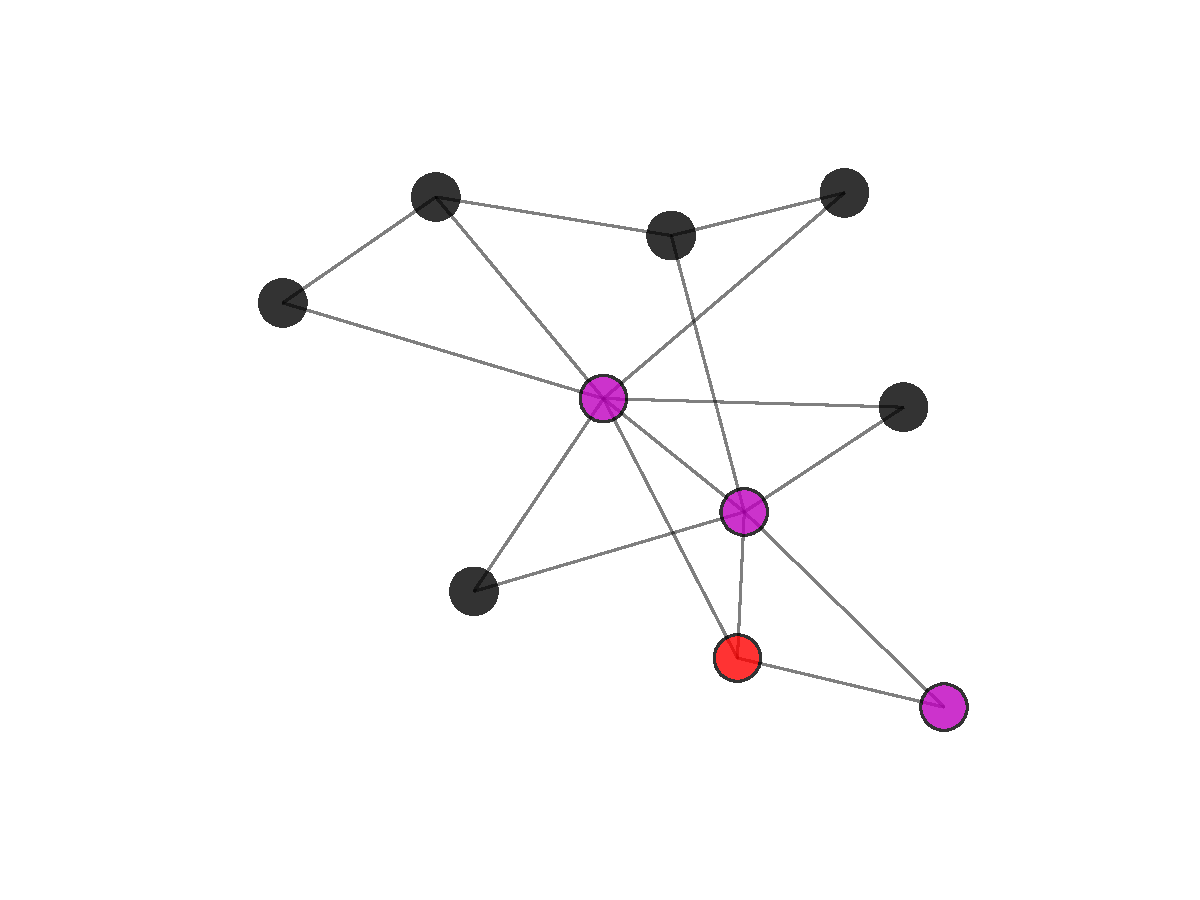
\includegraphics[width=0.4\textwidth]{labels_and_colors.pdf}	
	\end{figure}

Intermediate of the full information and the bandit setting
\vspace{0.7cm}

\textcolor{WildStrawberry}{\textbf{Challenge:}} leverage side observations in the setting where the graph is \textcolor{WildStrawberry}{random} and \textcolor{WildStrawberry}{changes at each iteration}.
\end{frame}

\begin{frame}{Random graph models}
\begin{columns}
	\begin{column}{.5\textwidth}
		\begin{figure}[ht]
			\centering
			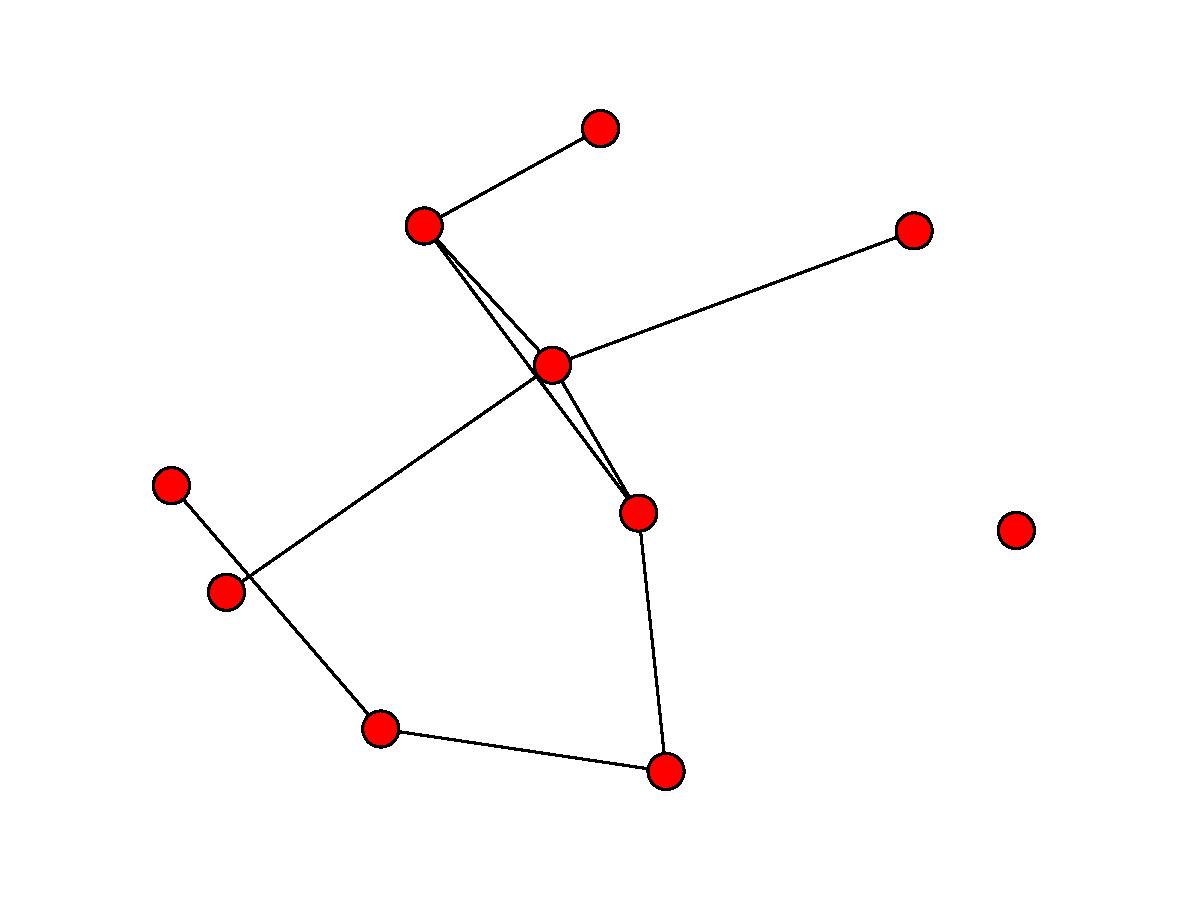
\includegraphics[width=\textwidth]{newER_graph_20.pdf}
			\caption{Edn\H{o}s R\'enyi}
		\end{figure}
	\end{column}
	\begin{column}{.5\textwidth}
		\begin{figure}[ht]
			\centering
			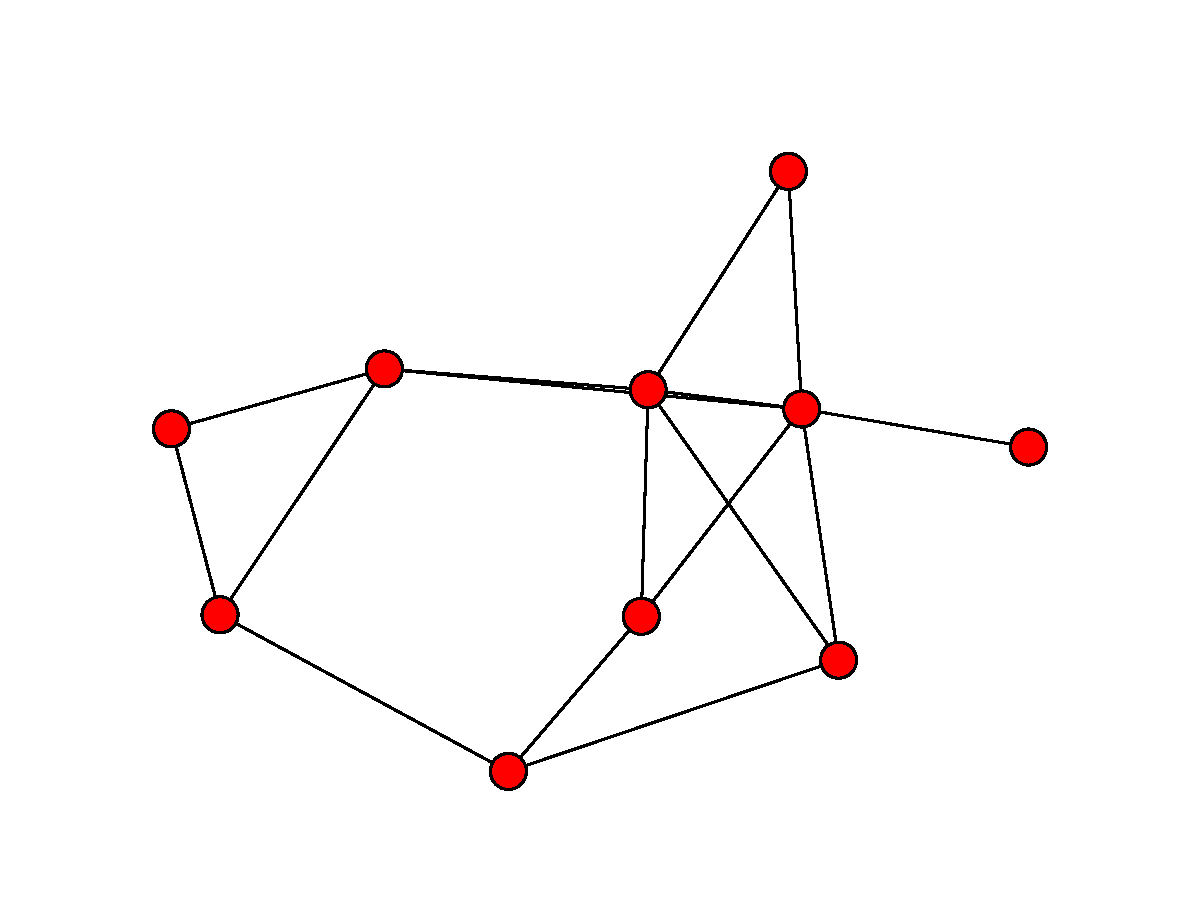
\includegraphics[width=\textwidth]{newBA_graph_2.pdf}
			\caption{Barab\'asi Albert}
		\end{figure}
	\end{column}
\end{columns}
\end{frame}

\section{Algorithms}
\subsection{Exp3}
\begin{frame}{Exp3: The algorithm}
Initialize $w_{i,0} = 1$
\begin{itemize}
\item Compute the new probabilities
\[
\hat{p}_{i,t} = (1 - \gamma) \frac{w_{i,t-1}}{\sum_{i=1}^N w_{i,t-1}} + \frac{\gamma}{N}
\]
\item pull one arm at random $I_t \sim \hat{p}_t$
\item observe losses $\ell_t$ following the random vector $O_t$
\item update weights
\[
w_{i,t} = w_{i, t-1} \exp(- \frac{\eta O_{i,t} \ell_{i,t}}{p_{i,t}})
\]
\end{itemize}
\textcolor{WildStrawberry}{Problem: } The correct normalizing factor should be $\mathbb{P}(O_{i,t}=1)$ instead of $p_{i,t}$ $\Rightarrow$ \textcolor{WildStrawberry}{\texttt{DuplExp3}}
\end{frame}

\subsection{DuplExp3}
\begin{frame}{DuplExp3: The idea}
The update formula should be $\hat{\ell}_{i,t}^* = \frac{O_{i,t} \ell_{i,t}}{\underbrace{p_{i,t} + (1-p_{i,t})\textcolor{WildStrawberry}{r}}_{o_{i,t}}}$. 

The r. v. $G_{t,i} \sim \mathcal{G}(o_{t,i})$ is used to  $1/o_{i,t}$, with $G_{t,i} \independent O_{t,i}$

To ensure independance, there are two distinct EXP3 alogorithms, $O_{t-1}$ is used to draw $G_{t,i} \sim \mathcal{G}(o_{t,i})$ \textbf{independently of} $O_{t}$.
\end{frame}

\subsection{Differences induces by the BA graph model}
\begin{frame}{Why DuplExp3 does not work as well on BA graphs}
\end{frame}

\subsection{BAexp3}
\begin{frame}{BAexp3: The algorithm}
\end{frame}


\section{Experimental results: observed regret curves}
\begin{frame}{Comparison of EXP3 and DuplEXP3 on ER graphs}
\end{frame}

\begin{frame}{Comparison of DuplEXP3 performance on ER and BA graphs}
\end{frame}

\begin{frame}{Performance of our algorithm for BA graphs}
\end{frame}

\section{Conclusion and future work}
\end{document}
